\documentclass[11pt,dvipdfm]{article}
%\documentclass[11pt]{article} %The above line must be used for your camera-ready submission, which requires %a latex -> DVI -> PDF compilation pipeline.  As a workaround while you are writing your paper, you could %comment it out and use this line instead, which is compatible with pdflatex.
\usepackage{deauthor,times,graphicx,hyperref} 
\usepackage{enumitem}

\begin{document}
\title{A Human-Centered Methodology for Creating AI FactSheets}
\author{John Richards, David Piorkowski, Michael Hind,\\Stephanie Houde, Aleksandra Mojsilovi\'c, Kush R. Varshney\\IBM Research AI\\ajtr@us.ibm.com, djp@ibm.com, hindm@us.ibm.com,\\stephanie.houde@ibm.com, aleksand@us.ibm.com, krvarshn@us.ibm.com}

\maketitle
\begin{abstract}
As artificial intelligence (AI) models and services are used in a growing number of high-stakes areas, a consensus is forming around the need for a clearer record of how these models and services are developed to increase trust.
  Several proposals for higher quality and more consistent AI documentation have emerged to address ethical and legal concerns
  and general social impacts of such systems.
  However, there is little published work on how to create this documentation.
  %%Over the course of our own work in this area, we have developed 
  In this paper we describe
  a methodology for creating the form of AI documentation we call FactSheets.
  This paper describes the methodology and shares the insights we have gathered while creating nearly two dozen FactSheets.   
  Within each step of the methodology, we describe the issues
  to consider and the questions to explore with the relevant people in an organization who will be creating and consuming AI facts.
  This methodology may help foster the creation of transparent AI documentation.
\end{abstract}

\section{Introduction}

Recent work has outlined the need for increased transparency in artificial intelligence (AI) for data sets \cite{gebru-2021,data-statements,HollandHNJC2018,dataset-nut-label-2gen-2020}, models \cite{model-cards}, and services~\cite{factsheets-2019}. Proposals in support of ethical and trusted AI are also emerging ~\cite{EuropeanCommission2020,raji2019ml,ieee-2017}. Although the specifics differ, all are motivated by the desire to define a set of attributes that capture essential details of how an AI model or service was developed and tested to better understand technical, ethical, and regulatory concerns.

Despite this work on transparent reporting mechanisms, there is little consideration of how to create this documentation. 
Determining \emph{what information} to include and \emph{how to collect} that information is not straightforward.
To our knowledge this is the first work outlining a methodology for creating this documentation.
We believe this methodology can promote the creation of useful AI documentation.

We have proposed a mechanism for AI documentation called FactSheets~\cite{factsheets-2019}. FactSheets take a more general approach to AI transparency than previous 
proposals~\cite{gebru-2021,data-statements,HollandHNJC2018,model-cards,EuropeanCommission2020,EuropeanCommission2021}
in several ways:\\

\begin{itemize}[noitemsep,nolistsep]
    \item FactSheets are
tailored to the particular AI model or service being documented, and thus can vary in content 

\item FactSheets are tailored to the needs of their target audience or consumer, and thus can vary in content and format, even for the same model or service

\item FactSheets capture model or service facts from the entire AI lifecycle

\item FactSheets are compiled from information generated by multiple contributors as they perform their actions throughout this lifecycle, thereby increasing the accuracy of these facts
\end{itemize}
\hspace{.2cm}

FactSheets can document AI services in addition to individual models. We think this is important for three reasons:\\

\begin{itemize}[noitemsep,nolistsep]
    \item AI services are the building blocks for many AI applications.
Developers call the service API and
consume its output. An AI service can be an amalgam of many models
trained on many datasets.  The models and associated datasets are (direct
and indirect) components of an AI service, but they are not themselves the
interface to the developer.

\item An expertise gap often exists between the producer and consumer of
an AI service. The production team leverages the
creation of one or more AI models and thus will mostly contain data
scientists. The consumers of the API services tend to be developers.
When such an expertise gap exists, it becomes more crucial to communicate the attributes of the service in a consumable way.

\item Services composed of trusted models may not necessarily be trustworthy, so
it is prudent to also consider transparency and accountability of
services in addition to datasets and models. In doing so, we take a
functional perspective on the overall service and can test for
performance, safety, and security aspects that may go beyond what is relevant for a
model in isolation.
\end{itemize}
\hspace{.2cm}

Our methodology is motivated by user-centered design principles~\cite{mao2005}, where input from multiple stakeholders is collected to inform design. Although this takes more time than a single person designing the documentation, it is significantly more likely to meet the needs of FactSheet consumers \cite{madaio2020}.
This paper focuses on a specific form of AI documentation, FactSheets, but the techniques can be applied to other forms of AI (or even non-AI) documentation. Note, also, that our discussion centers on business applications of AI but the techniques can be applied to creating documentation for AI outside of this setting.

Before we describe our methodology in detail, we first highlight a few key concepts.  
Section~\ref{sec-lifecycle} describes the AI lifecycle, summarizing the relevant roles and workflow for the construction and deployment of an AI model or service.
Section~\ref{sec-FactSheets} describes the concept of a FactSheet and motivates the need for a FactSheet Template. Section~\ref{sec-methodology} presents our seven-step methodology for constructing useful FactSheets.
Section~\ref{sec-final} presents further guidance for those organizations planning to create FactSheets.
Section~\ref{sec-harm-safety} discusses how the methodology can help to address the needs of consumers with regards to the potential safety and harm of AI.
Finally, Section~\ref{sec-practice} touches on what we are finding as FactSheets are put into production use.

\section{The AI Lifecycle}
\label{sec-lifecycle}
The AI lifecycle includes a variety of roles, performed by people with different specialized skills and knowledge that collectively produce an AI model or service. Each role contributes in a unique way, using different tools. Figure~\ref{fig:lifecycle} specifies some common roles.

\begin{figure}
    \centering
    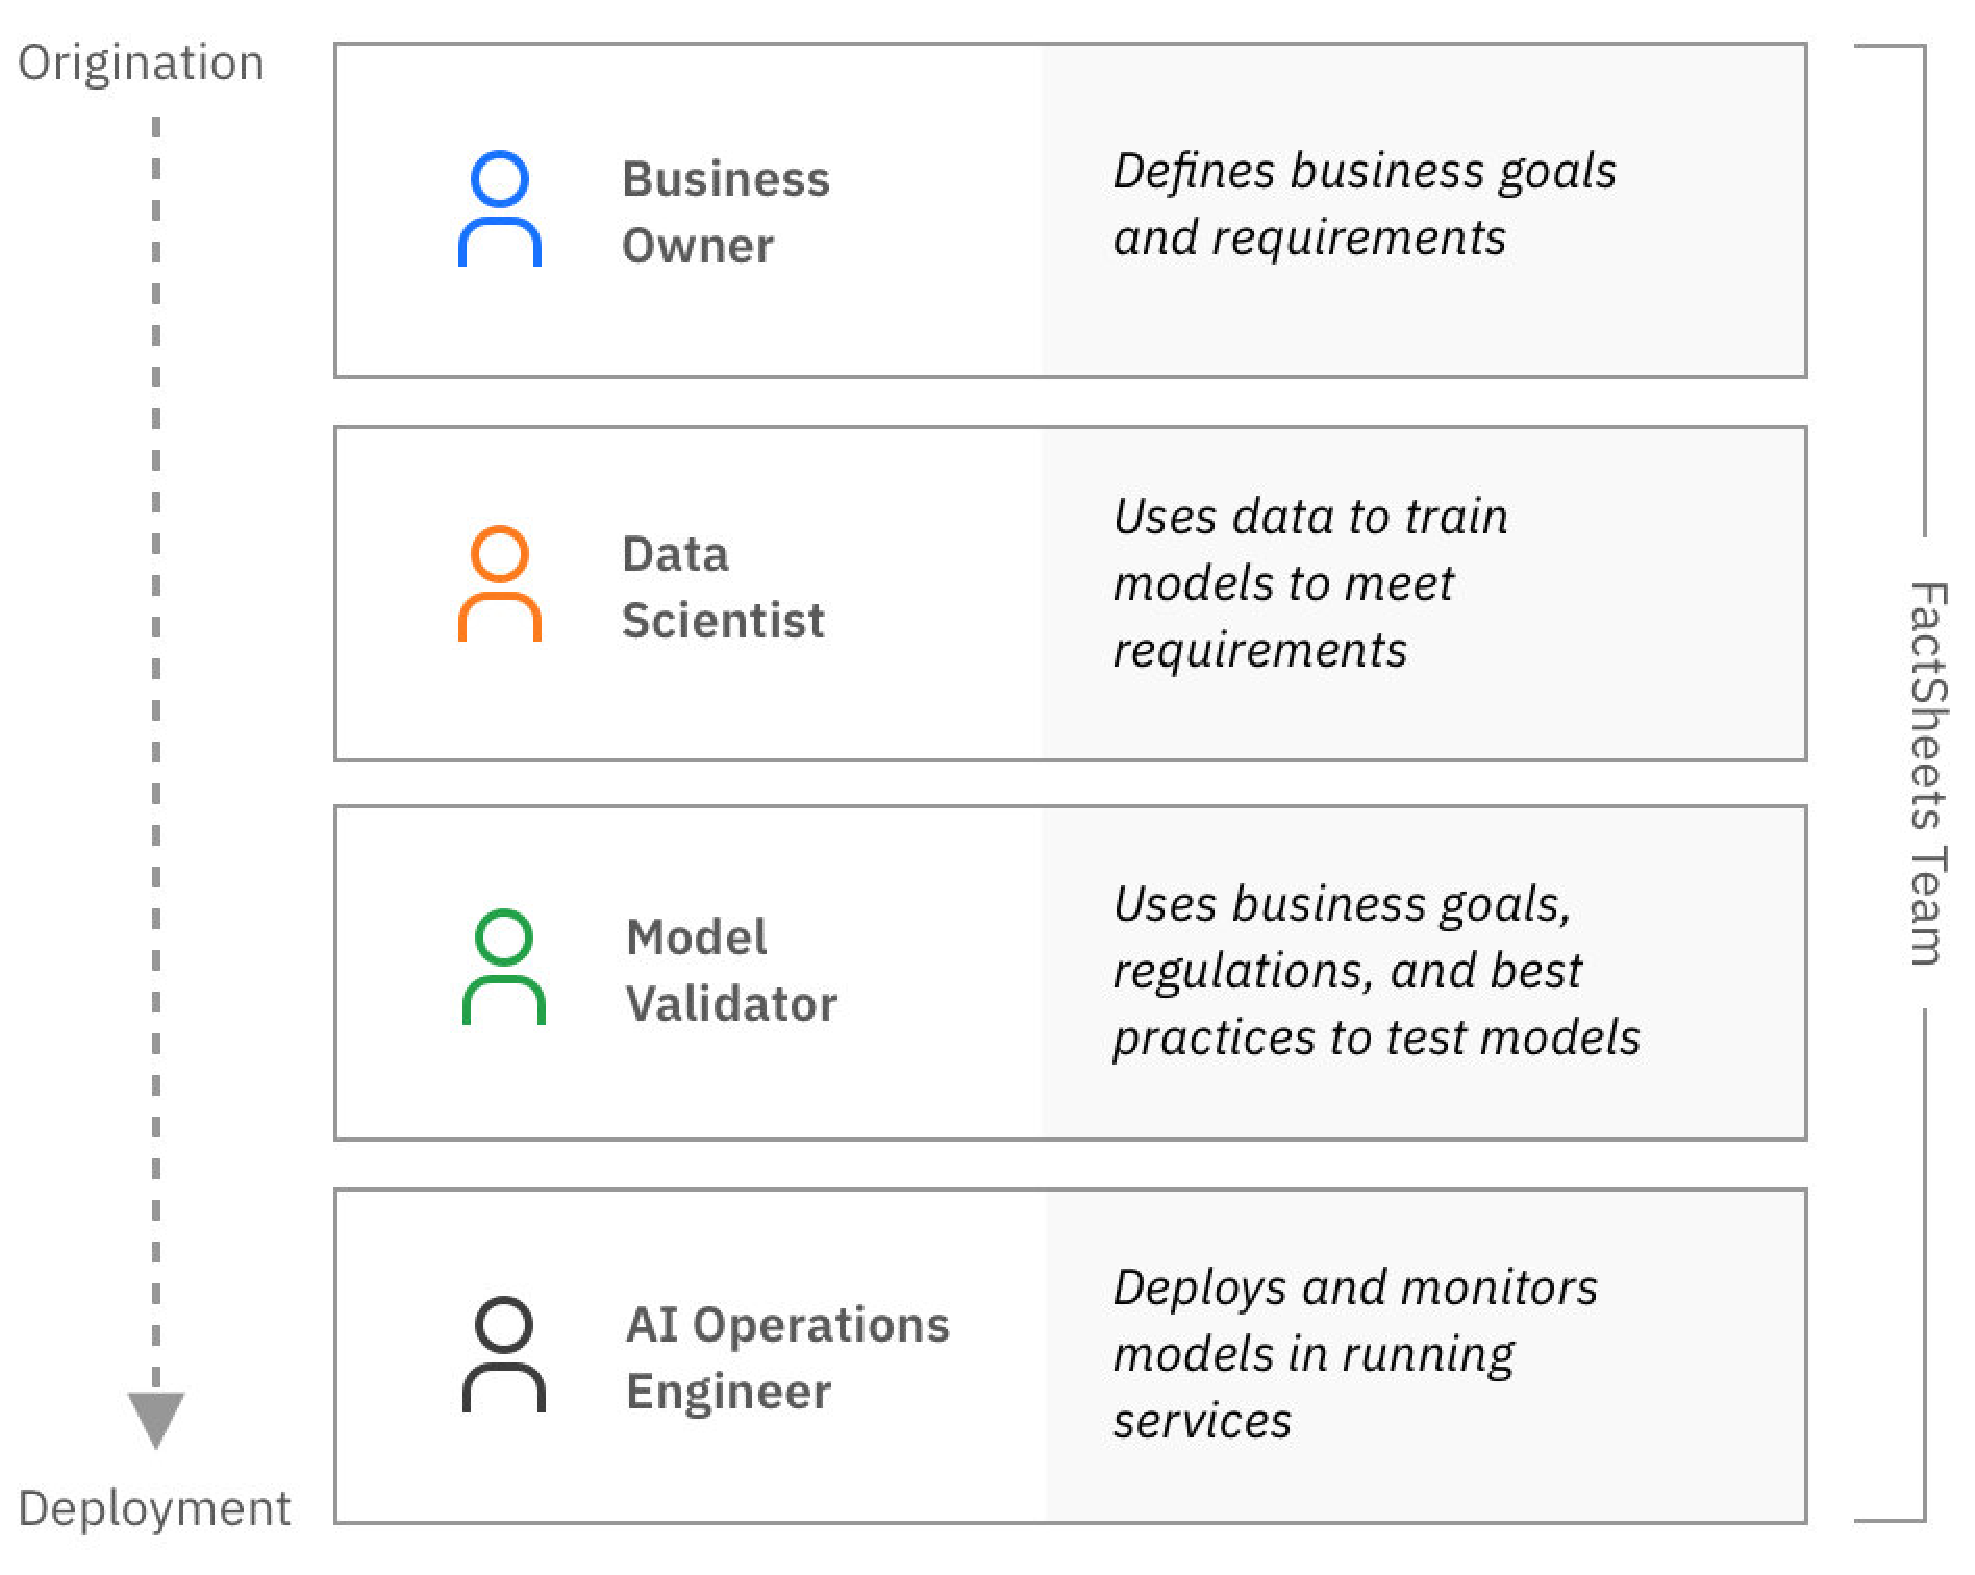
\includegraphics[width=0.45\textwidth]{figs/Img1_Roles.eps}
    \caption{Key roles in a typical AI lifecycle}
    \label{fig:lifecycle}
\end{figure}

The canonical process starts with a business owner who requests the construction of an AI model or service. The request includes the purpose of the model or service, how to measure its effectiveness, and any other constraints, such as bias thresholds, appropriate datasets, or the required levels of explainability and robustness.

The data scientist uses this information to construct a candidate model by using, most typically, a machine learning process. This iterative process includes selecting and transforming the dataset, discovering the best machine learning algorithm, tuning algorithm parameters, etc. The goal is to produce a model that best satisfies the requirements set by the business owner.

Before this model is deployed it often must be tested by an independent person, referred to as a model validator in Figure 1.
This role, often falling within the scope of model risk management~\cite{model-risk-mgmt}, 
third party testing~\cite{3rd-party-testing,eu-testing}, or certification~\cite{certification,eu-testing}, is similar to a testing role in traditional software development. 
A person in this role may apply a different test dataset to the model and independently measure metrics defined by the business owner. 
The person may also develop a "challenge" model to see if a simpler, and thus, less risky, solution could solve the same problem.
If the validator approves the model, it can be deployed.

The AI operations engineer is responsible for deploying and monitoring the model in production to ensure it operates as expected. This can include monitoring its performance metrics, as defined by the business owner. If some metrics are not meeting expectations, the operations engineer is responsible for taking actions and informing the appropriate roles.

AI lifecycles will include iteration within a role (a data scientist, building many models before passing it to a validator) or between roles (an operations engineer sending a model back to a data scientist because it is performing poorly).
More sophisticated lifecycles will likely have additional roles. A common pattern is for a model to be combined with other models or human-written code to form a service. In such a case the validator's role may be extended to also validate the full service.

A model is not a static object in the lifecycle, and thus, a FactSheet must incorporate the facts and lineage from all phases of the ``life of the model''.  This will introduce transparency not only into how the model was built and what it does, but also how it was tested, deployed, and used.

\section{FactSheets and Templates} \label{sec-FactSheets}

\textbf{FactSheets}~\cite{factsheets-2019} are a collection of information 
about how an AI model or service was developed and deployed.  
% This information includes information gathered, ideally, throughout the AI lifecycle. 
FactSheets summarize the key characteristics of a model or service for use by a variety of stakeholders. We have previously summarized the difficulties developers face when creating FactSheets~\cite{experiences-2020}. 
%%MH This paper summarizes the best practices we have discovered along the way. 
This paper describes the best practices we have developed in the process of creating FactSheets for nearly two dozen models.
These include FactSheets for standalone models as well as services that encapsulate one or more models.
%as well as multimodel ensembles or multimodel collections. 
They cover a wide range of application areas including text analysis and generation, language translation, object detection, object classification, audio signal classification, weather forecasting, agricultural crop yield prediction, and facility energy optimization.   

This work has demonstrated that although FactSheets will contain some common elements, different FactSheets will generally contain different information, at different levels of specificity, depending on domain and model type. They will also contain different information for different industries and the different regulatory schemes within which these industries operate. 

Within a particular domain or organization, FactSheets will also take on different forms, and contain different content, for different purposes. Model validators may need detailed information on data selection and cleaning, feature engineering, and accuracy and bias metrics. Business owners may need information on whether a deployed model is meeting business needs. Regulators may need a report detailing how a model complies with established practices and metrics related to safety, bias, and harm.
Thus, although there is a strong desire to create a standard template for all FactSheets, we believe this diversity illustrates that for FactSheets, \textbf{one size does not fit all}. 


We believe that standards will eventually emerge and, like nutrition labels, be useful for some purposes. 
In the foreseeable future, however, many kinds of FactSheets will be created. 
We have created the notion of \textbf{FactSheet Templates} to manage this diversity. A FactSheet Template can be thought of as specifying the categories or types of information that will be collected and displayed during and after AI development. Any given lifecycle will likely have multiple templates since different people will likely want to see different information, for different purposes, at different points in time. A large part of the job of creating FactSheets is designing the appropriate FactSheet Template(s). This is a prime focus of Section~\ref{sec-methodology}.



% -------------------------------------- FactSheet Methodology ---------------------------------------
\section{FactSheet Methodology}
\label{sec-methodology}
We now describe our seven-step methodology for the construction of useful FactSheets.
For expository purposes, the steps shown in Figure~\ref{fig:flowchart} are presented as though they flow in a single stream from beginning to end. The reality is that FactSheet production is highly iterative, especially in the early days of FactSheet adoption within an organization.

\begin{figure}
    \centering
    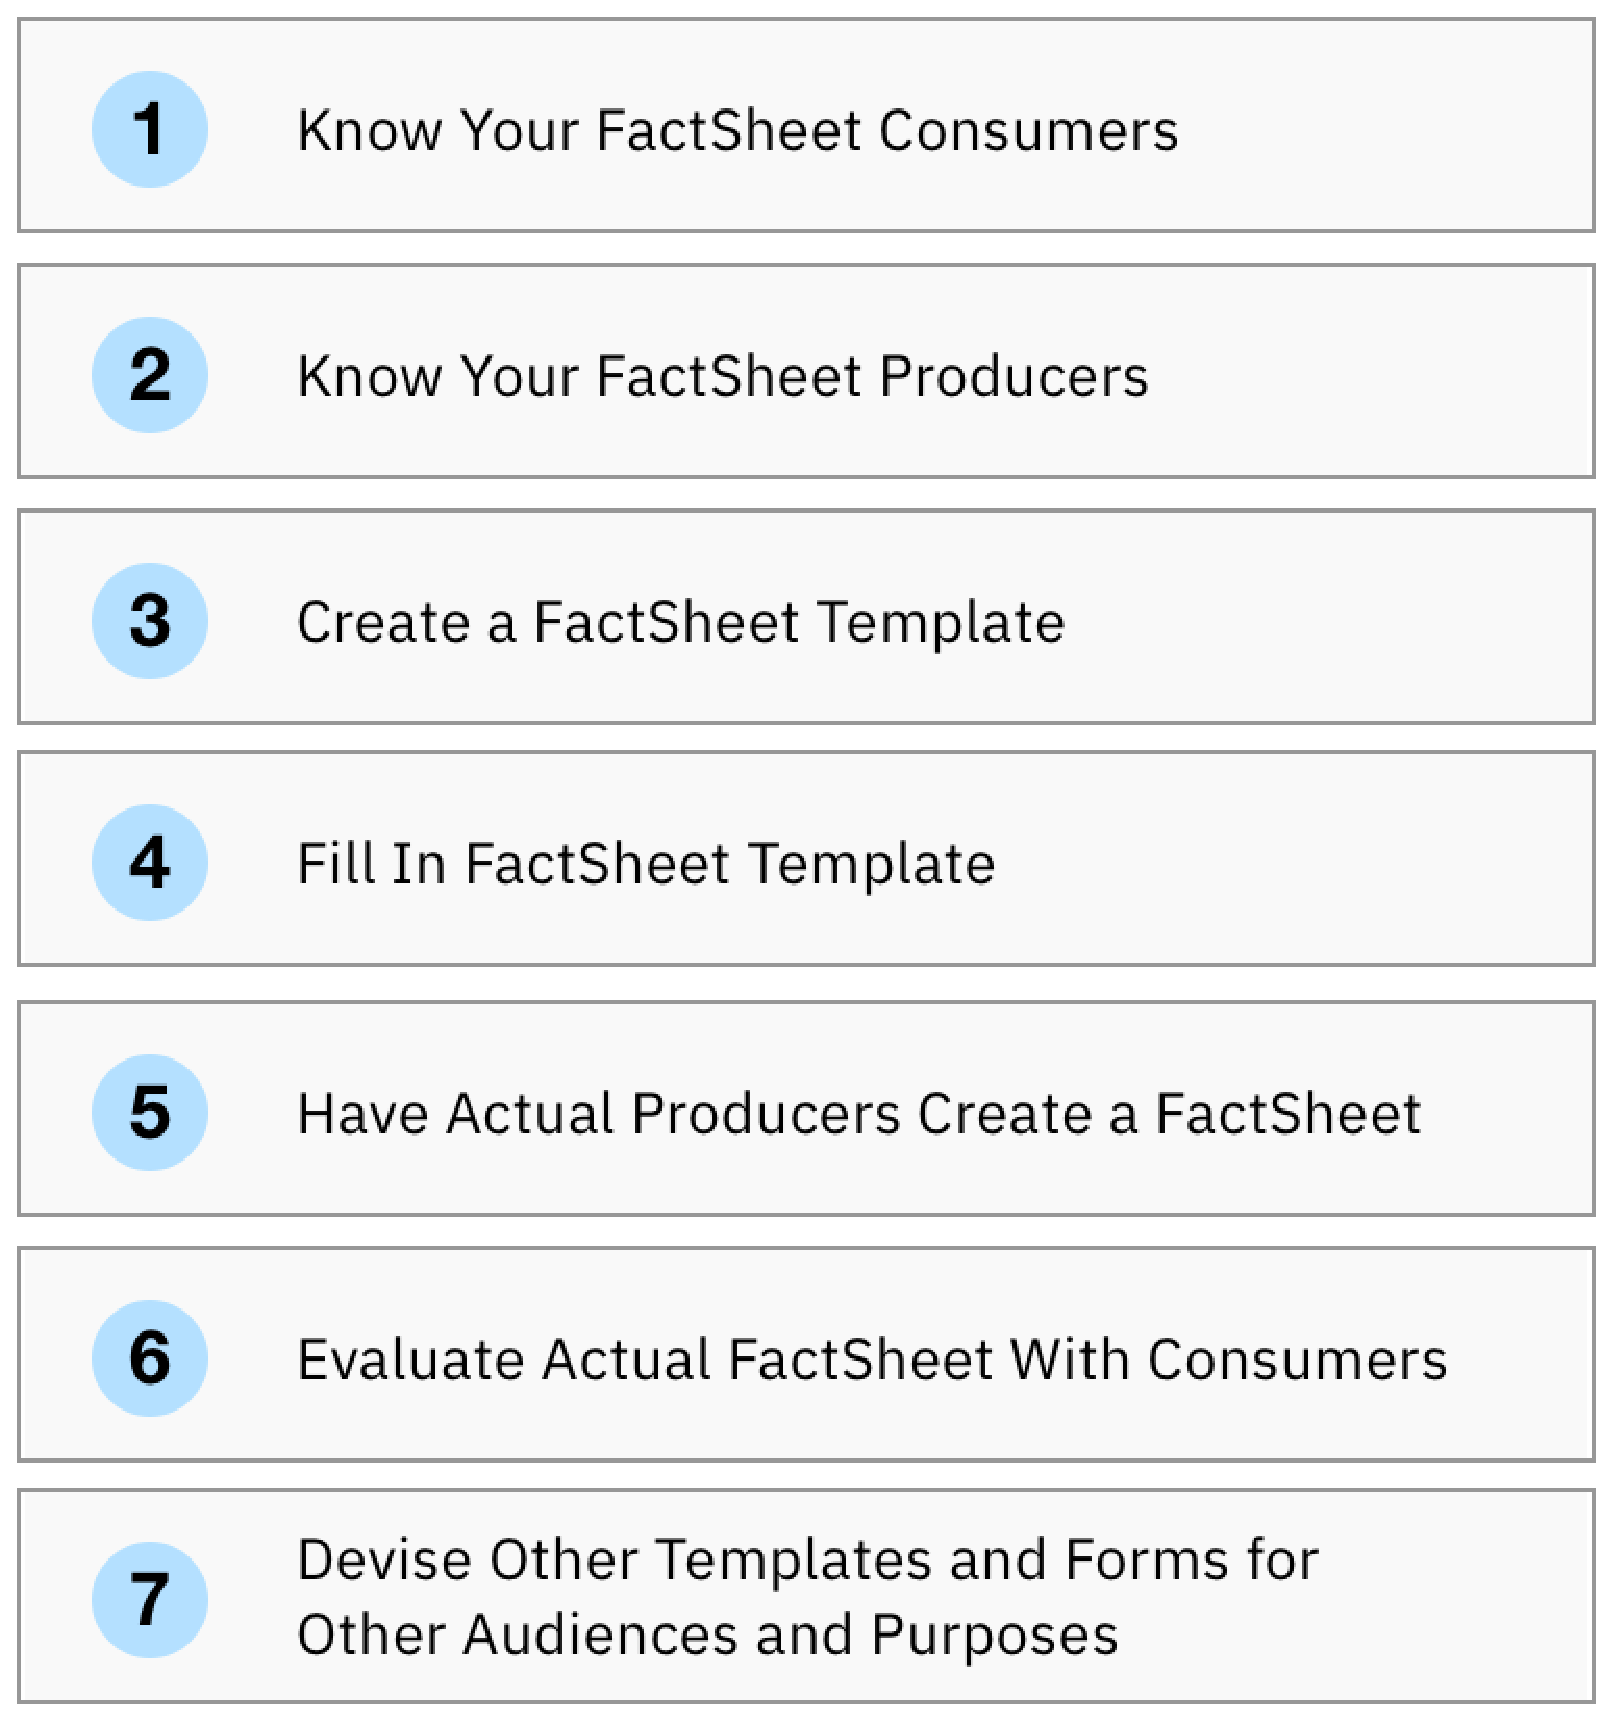
\includegraphics[width=0.45\textwidth]{figs/Img2_Steps.eps}
    \caption{Steps to produce useful FactSheets}
    \label{fig:flowchart}
\end{figure}

Each step lists the key roles involved. In addition to the more typical roles shown in Figure~\ref{fig:lifecycle}, an additional role is identified, namely the ``FactSheets Team''. This team is responsible for designing and implementing the FactSheets process within the organization. The first three steps will be driven by this team as they interview potential FactSheet consumers and producers and design the first FactSheet Template. Step 4 will largely be performed by the FactSheets Team but will benefit from the involvement of those with direct knowledge of the model or service being documented. This step may involve several iterations and informal trials with potential consumers and producers. In Step 5, FactSheet producers will generate an actual FactSheet. In Step 6, FactSheet consumers will assess the quality and usefulness of this FactSheet. The FactSheets Team will be involved in these latter steps as well but will rely heavily on others to produce and attempt to consume actual content. In Step 7, the FactSheets Team repeats the process to increase coverage and value.

To simplify the presentation in the following steps we focus on one fact producer, ``Priya'', and one fact consumer ``Carmen''. Priya is a data scientist who will generate facts about how she created her model. Carmen is a model validator who will assess the model Priya created on various dimensions including quality, simplicity, and potential risk. Of course, Priya may also be a consumer of facts produced earlier by those who assembled the training data she uses. Similarly, Carmen may be a producer of facts for those who make the final decision on deployment readiness of the model she validates.
%% mention external consumers
Although our consumer in this example, Carmen, is part of the AI lifecyle, there are other possible documentation consumers that are outside of the AI lifecycle, such as end users (e.g., a loan officer), affected users (e.g., a loan applicant), or regulators.  The same methodology would apply in these cases as well.

This may seem like a lot to think about, especially when there are multiple roles to understand and a desire to  sample multiple representative users within each role. But the important thing is to start. Find one person performing each role (some people will be performing more than one role). Spend 30 minutes in conversation with each of them. If needed, find more than one person to explore areas that are still unclear after the first conversation. To speed things up, consider bringing potential producers and consumers together in conversation at any point in this process. They may quickly converge on what information is needed and how it can be produced in a cost-effective way. 



\subsection{Step 1: Know Your FactSheet Consumers}

\begin{itemize}[noitemsep,nolistsep]
    \item Who: FactSheets Team (with potential consumers)
    \item What: Gather the information needs of potential FactSheet consumers
\end{itemize}
\hspace{.2cm}

FactSheets are produced so that they can be consumed. Understanding the information needs of FactSheet consumers is the first and most important task. Here are some of the questions to consider in this first step (with Carmen, a model validator, as the illustrative consumer):\\

\begin{enumerate}[noitemsep,nolistsep]
\item What does Carmen currently do when she performs her role?
\item What is Carmen going to be asking for when looking at a FactSheet?
\item What decisions will she be making based on the information presented?
\item How is the FactSheet going to help her do her job more effectively?
\item What are the most important pieces of information that Carmen needs to know?
\item What is Carmen's level of expertise in general data science?
\item How is Carmen's expertise going to affect the information presented?
\item Will there need to be additional definitions for terms that Carmen is unfamiliar with?
\item What is Carmen's level of expertise with respect to the model algorithms being used?
\item What explanations about the model's algorithm or results is Carmen going to need?
\item What is Carmen's level of expertise in the problem domain?
\item How is that going to affect the information presented?
\item Will Carmen need help in mapping general knowledge of the problem domain to the particular inputs, outputs, or performance indicators associated with this model?
\item Is Carmen aware of issues related to model risk, potential harm, and regulatory compliance?
\item What information is needed to assess these issues?
\end{enumerate}
\hspace{.2cm}

\subsection{Step 2: Know Your FactSheet Producers}

\begin{itemize}[noitemsep,nolistsep]
    \item Who: FactSheets Team (with potential producers)
    \item What: Gather the kinds of information FactSheet producers might generate
\end{itemize}
\hspace{.2cm}

Some facts can be automatically generated by tooling. Some facts can only be produced by a knowledgeable human. Both kinds of facts will be considered during this step. Here are some of the questions we might explore with Priya (a data scientist) about the facts she could usefully generate during the creation of a model:\\

\begin{enumerate}[noitemsep,nolistsep]
\item What facts does Priya wish she could conveniently record about the models she develops? It is often helpful to ask about the most recent model, or a model that was particularly important, or a model that was exceptionally difficult to produce, rather than discussing models in general.
\item What did Priya do during the creation of this model that is otherwise unknown to others?
\item Are there general facts about the data, the features, the model algorithm, or the training and testing Priya performs that are important to note? Why?
\item What model-specific knowledge does she have that may not be obvious to others?
\item What domain-specific knowledge does Priya have that may not be obvious to others?
\item Does Priya know who will be consuming the facts she produces? We will assume it is Carmen in this particular case. Does Priya know Carmen? Have they talked about what Carmen needs to know?
\item Is Priya aware of issues related to model risk, potential harm, and regulatory compliance?
\item What information will be needed by others to assess these issues?
\end{enumerate}
\hspace{.2cm}

\subsection{Step 3: Create a FactSheet Template}

\begin{itemize}[noitemsep,nolistsep]
    \item Who: FactSheets Team
    \item What: Define the topics and questions to be included in FactSheets
\end{itemize}
\hspace{.2cm}

What is learned in the first two steps leads directly to the most important part of creating FactSheets, namely the creation of a FactSheet Template. As discussed in Section~\ref{sec-FactSheets}, a FactSheet Template will contain questions. Each individual FactSheet will contain the answers to these questions. For example a template may start with the question ``What is this model for?''. It may then expand on that question by asking where the model is well-suited and where the model is ill-suited.

The information gathered in the first two steps will inform the creation of this FactSheet Template. You may find that details about how a model is created are much less important in your organization than information about risk assessments and regulatory compliance. Or you may find that detailed questions about robustness against adversarial attacks are needed because of the nature of the models you create or the high-stakes domains within which they are used.

Here are some of the questions to consider in creating the first iteration of a FactSheet Template. Again, this is cast in terms of Carmen's needs for information and Priya's ability to produce that information, but similar questions will apply to many of the roles in the AI lifecycle
or external consumers of the AI documentation.\\

\begin{enumerate}[noitemsep,nolistsep]
    \item What are the topics or categories of information needed?
    \item Do some of these categories have subcategories?
    \item What is a meaningful name for each category or subcategory?
    \item What kinds of information should be included in each category? For example, Carmen may want to group all the model performance metrics within a category called ``Model Performance''. Information about the representativeness of the training data might be grouped with information on the sensitivity of the model to drift in a category called, ``Potential Sources of Error''.
    \item How should each question in a category be worded so as to be both understandable and evocative for Priya? The goal here is to encourage fact producers to answer in ways that are concise, germane, and understandable.
    \item Where will the answer to a question come from? Will it be generated automatically by a tool or entered by a knowledgeable human? If the former, will Priya have some control over the frequency of fact generation or the granularity of recorded facts? If the latter, will Priya be given hints or examples of the kind of answer that would be satisfactory?
    \item Are there any regulatory, legal, or business concerns that need to be considered when answering the questions in this template?
    \item Are there different presentation formats needed for this information (for example, a short tabular summary of just key facts, or a slide format for presentations to review boards)? AI FactSheets 360~\cite{fs360} shows three different formats that might be useful.
    \item In addition to the human-readable content, is there a need for machine-readable content that Priya might generate?
\end{enumerate}

\subsection{Step 4: Fill In FactSheet Template}

\begin{itemize}[noitemsep,nolistsep]
    \item Who: FactSheets Team
    \item What: Informally assess FactSheet Template by trying to fill it in
\end{itemize}
\hspace{.2cm}

This step is where you will attempt to fill in your FactSheet Template for the first time. As you do this, informally assess the quality of the template itself. While this assessment is not a substitute for further work with Priya and Carmen (to follow), it may quickly highlight where improvements are needed. In doing this assessment, try to reflect on the template and the FactSheets it will generate from Carmen's and Priya's points of view. Ask yourself, or other members of your FactSheets Team, the following questions:\\

\begin{enumerate}[noitemsep,nolistsep]
\item Knowing what Carmen knows, will she be able to understand the information that filled-in FactSheets will include?
\item Are there details needed by Carmen that will be missing in these FactSheets?
\item Is there specialized language that Carmen will be unfamiliar with?
\item Will the information allow Carmen to make the decisions she needs to make?
\item How are these FactSheets going to help Carmen do her job more effectively?
\item What might we do to encourage Priya to answer questions in ways that provide what Carmen needs?
\end{enumerate}

\subsection{Step 5: Have Actual Producers Create a FactSheet}

\begin{itemize}[noitemsep,nolistsep]
    \item Who: Business Owner, Data Scientist, Model Validator, AI Operations Engineer (and others as defined within your organization's AI lifecycle)
    \item What: Populate a FactSheet Template with actual facts
\end{itemize}
\hspace{.2cm}

At this point you have a solid template and a good sense of how it might be used to create FactSheets. The next step is to have actual fact producers fill in the template for their part of the lifecycle. If there is a question in the template about model purpose, find someone who would actually be entering that information and have them answer the question. Ask a data scientist to answer the questions related to the development and testing of an actual model. If this model was validated, ask the model validator to enter information about that process. 
Similarly, have a person responsible for model deployment answer those questions.
If the lifecycle is not that structured, have the person responsible for most of the work create this FactSheet. 

We have found this step to be highly iterative. You can expect sections of your template to be expanded, compressed, or eliminated altogether. Individual questions will be refined within these sections. Stay alert for ideas or helpful hints about other fact producers that may surface. Follow these leads later. The goal here is to create a FactSheet that is ready for evaluation by consumers in the next step. Take the time to get this FactSheet to a level of quality and completeness that will make this next evaluation meaningful.

\subsection{Step 6: Evaluate Actual FactSheet with Consumers}

\begin{itemize}[noitemsep,nolistsep]
    \item Who: Business Owner, Data Scientist, Model Validator, AI Operations Engineer (and others as defined within your organization's AI lifecycle)
    \item What: Assess FactSheet quality with those who will be consuming FactSheets in production
\end{itemize}
\hspace{.2cm}

In this step we conduct an assessment of the quality and completeness of the actual FactSheet produced in the previous step. If the FactSheet is intended to be used by multiple roles (not uncommon), evaluate it separately for each role. To make each evaluation meaningful, ensure you have agreement with respect to the purpose of the FactSheet. Ask the consumer to imagine using this FactSheet to actually perform their work.

Each evaluation consists of two parts. The first focuses on the content in the FactSheet. The second focuses on the way in which information is presented.

\paragraph{Content Evaluation:} The goal of this part of the evaluation is to see how well the content of the FactSheet meets the specifically-designed-for information needs of the consumer. Ask your consumer to go through the FactSheet item by item with their information needs in mind and identify the following:\\

\begin{enumerate}[noitemsep,nolistsep]
    \item What information is missing?
    \item Why is that missing information important to include?
    \item How would they like this information presented?
    \item Can they give an example?
    \item What information is extraneous?
    \item Why is that information extraneous?
    \item What information is confusing or hard to understand?
    \item Why is that information hard to understand?
    \item How can that information be made more understandable?
    \item Can they give an example?
    \item Was the organization of information sensible?
    \item If not, what would they change?
\end{enumerate}
\hspace{.2cm}

Have the consumer rank the information presented in this FactSheet from most important to least important. Remember to include the information that was noted as missing in this ranking. If time permits, have them share their views about the FactSheet with your larger group. Encourage discussion and ask questions about any unexpected findings, which can often identify gaps in the underlying lifecycle process or confusion about roles. Addressing these gaps can pay large dividends.

\paragraph{Presentation Evaluation:} The goal of this part of the evaluation is to see if the way that information is \textit{presented} meets the specifically-designed-for information needs of the consumer. Since some of the information you collect may be visual, make sure to allow for that type of feedback. Ask each consumer to go through the FactSheet item by item with their information needs in mind and identify these things:\\

\begin{enumerate}[noitemsep,nolistsep]
    \item Is this information presented in an unexpected way?
    \item How can the information be presented differently?
    \item Why is this alternative a better way to present this information?
    \item Can they draw or describe an example?
    \item If the information presentation includes interactive elements, are they useful?
    \item How can they be made more useful?
    \item Why is that more useful?
    \item If they could add or change the way that information is presented, how would they?
    \item Why is this addition or change an improvement?
    \item Is this, overall, the right format for presenting this information?
    \item What format would be more suitable?
    \item Why is that format more suitable?
\end{enumerate}

\subsection{Step 7: Devise Other Templates and Forms for Other Audiences and Purposes}

\begin{itemize}[noitemsep,nolistsep]
    \item Who: FactSheets Team (and others as appropriate)
    \item What: Evolve existing templates and create new ones
\end{itemize}
\hspace{.2cm}


By now you will have created a refined FactSheet Template for use by others. They will be able to create useful and consumable FactSheets with that template. But there is more to do. There may be other consumers that need to be supported. Perhaps it is time to turn from an inward focus to an outer one, crafting templates for FactSheets to be consumed by external review boards or regulators. Or it may be time to support other stakeholders not directly involved in the AI lifecycle, such as sales personnel or the ultimate consumers of an AI service. Other formats for the same content may need to be created as well. The above steps can be followed once again. You will have  learned a surprising amount about \textit{how} to create FactSheet Templates and FactSheets from having gone through this process once. It will go faster and more smoothly now.

We encourage an ongoing process of reflecting on how well FactSheets support your AI lifecycle once they are fully incorporated and in routine use. Consider how they might be improved. Perhaps a new business opportunity in a new domain has developed or new types of models are being created that capitalize on new algorithmic research. If so, it may be time to refine existing FactSheet Templates or create new ones.

\section{Further Guidance}
\label{sec-final}

We have observed ~\cite{experiences-2020} that producers of FactSheets have a hard time imagining what consumers of FactSheets need to know and how best to provide that information. Model developers, for example, may have a sophisticated understanding of the algorithmic basis for a model, but may describe the model or its performance in ways that assume far too much knowledge on the part of a FactSheet consumer. Consumers may not really know what information they need to support their work without somewhat structured reflection. Our methodology addresses these gaps by applying a user-centered design process \cite{mao2005} to the task of creating useful AI documentation. This process need not be time consuming and expensive. Even talking with a few potential FactSheet consumers and producers will be helpful.

It should be obvious at this point that following this methodology will not lead to a single FactSheet Template across the vast array of organizations creating AI models and services. The methodology \textit{will}, however lead to FactSheets that fit the needs of a particular organization and provide real value to the corresponding AI development, deployment, and monitoring teams.

To put it a different way, one size will not fit all, at least if you dive below a short nutrition-label-like form to something that provides useful detail to all the lifecycle roles in a real organization. Even FactSheets developed with the same template will differ in interesting ways. For example, some models will have FactSheets with extensive sections on bias and fairness testing with respect to protected populations. Other models will have FactSheets for which fairness and bias considerations are truly not applicable. Within some regulated industries, FactSheets may run to a hundred or more pages whereas the FactSheet produced by a startup company providing an AI component for visual object detection may be little more than a statement of purpose, inputs, and outputs.

An extension beyond user-centered design is \emph{participatory design}, which invites not only the producers and consumers within the organizations's AI development team to contribute to the process, but also the communities affected by the deployed model or service, such as applicants or patients \cite{lee2019we,prabhakaran2020}. Moreover, by including people with lived experience of marginalization, who have an epistemic advantage in spotting potential harms, you will obtain a more comprehensive FactSheet template than if you did not have their participation \cite{fazelpour2021}.

This methodology for creating FactSheets may seem like a lot of work. Following these steps \textit{will} take more time than just having a single person write a FactSheet Template based on a limited understanding of the actions and information needs within your organization. But failing to perform these steps will incur ongoing costs in poor documentation, repeated requests between team members for missing information, insufficient testing based on faulty assumptions about data or model structure, sub-optimal business results, and exposure to unnecessary risk.

We have found that following these steps with even a small number of people, where
there is perhaps only one representative for each stage in a lifecycle, will pay dividends. We have also found that
iterating quickly, rather than spending substantial time trying to attain perfection within each iteration, will shorten the overall time needed.

\section{Harm and Safety}
\label{sec-harm-safety}
The increasing use of AI systems in high-stakes decision making has
underscored the importance of transparent reporting mechanisms. These mechanisms, including FactSheets, can lead to better understanding, and more effective mitigation of any harm or safety issues in the system, such as bias, vulnerabilities to adversarial attacks, or other undesirable societal impacts. 
For example, a section that describes a detailed analysis of bias in the training dataset can help illuminate if the system is appropriate for a particular use case.

%% One example may be a bias section that explicitly points out implicit gender bias in the data set, explains the mitigation strategy to address the bias and also presents before/after results that indicate a successful bias mitigation.

This paper describes a methodology for producing a useful transparent reporting mechanism for AI systems.  This methodology can contribute to the identification of potential harm and safety issues. The methodology does this by:
\\
\begin{itemize}[noitemsep,nolistsep]
\item Explicitly including multiple FactSheet consumers and producers in FactSheet requirements gathering (Steps 1--2) 
\item Asking questions about their concerns for harm and risk (Steps 1--2) 
\item Providing a feedback mechanism to allow further input (Step 6)
\item Including a broad range of perspectives in the development of FactSheets (Steps 1--7)
\end{itemize}
\hspace{.2cm}


This process will increase the likelihood that FactSheets will provide the information needed to understand and mitigate potential harm or safety issues with an AI system.
  
\section{In Practice}
\label{sec-practice}
% This is all coming out super vague since I don't want to mention specific counts or quotes. @John, I'll leave it to you to tell me if something needs to be expanded or cut.
We have begun evaluating the FactSheets methodology across three teams within our company and have received strong positive feedback and calls for widespread adoption for both new and existing models and services. One early benefit has become evident from the work carried out by fact producers, who were primarily data scientists. They found that the step of identifying consumers and their documentation-related use cases provided them with a perspective and a sense of purpose that was lacking in their prior documentation efforts. They described how having a persona (or sometimes a specific person) in mind enabled them to more carefully shape their documentation to meet known needs, a strategy used by data scientists more generally when communicating about their models~\cite{piorkowski2021ai}. By having specific users in mind, data scientists were able to constrain \textit{what} facts to document and \textit{how} to present them, lessening the uncertainty that they reported experiencing in the past.

The benefits of the FactSheet methodology do not come without costs. Our FactSheet creators spent up to 24 working hours crafting a complete FactSheet, with roughly half that time spent gathering feedback from consumers and iterating on content to make it more consumable. These costs can be reduced with better technology to support the creation and curation of facts. But we note that the multidisciplinary nature of AI model development, with each role having their own distinct knowledge, information needs, and preferred tools for accomplishing their work, will continue to require a focus on collaborative activities with their attendant costs and complexities (such as scheduling meetings). Bridging the gap between roles while addressing the back-and-forth, iterative nature of creating FactSheets remains a challenge to be overcome.\footnote{An earlier version of this paper~\cite{FactSheets-Methodology-arxiv-2020}
includes two illustrative FactSheet templates created using this methodology.  The templates are for the same model, but for two different consumers, illustrating the generality of the approach.}


\vspace{-.1cm}
%\bibliographystyle{ACM-Reference-Format}

%% MH: Journal requires refs to be in tex file.
%% So, I took the bbl file from overleaf and pasted it below.
%% If we make any updates to references we need to uncomment the
%% 2 lines below and remove the bib stuff below and add the new
%% bbl contents
% \bibliographystyle{abbrv}
% \bibliography{refs2}

\begin{thebibliography}{10}

\bibitem{factsheets-2019}
M.~Arnold, R.~K.~E. Bellamy, M.~Hind, S.~Houde, S.~Mehta, A.~Mojsilovi{\'c},
  R.~Nair, K.~N. Ramamurthy, A.~Olteanu, D.~Piorkowski, D.~Reimer, J.~Richards,
  J.~Tsay, and K.~R. Varshney.
\newblock {FactSheets}: Increasing trust in {AI} services through supplier’s
  declarations of conformity.
\newblock {\em IBM Journal of Research \& Development}, 63(4/5), Sept. 2019.

\bibitem{data-statements}
E.~M. Bender and B.~Friedman.
\newblock Data statements for natural language processing: Toward mitigating
  system bias and enabling better science.
\newblock {\em Transactions of the Association of Computational Linguistics},
  2018.

\bibitem{dataset-nut-label-2gen-2020}
K.~S. Chmielinski, S.~Newman, M.~Taylor, J.~Joseph, K.~Thomas, J.~Yurkofsky,
  and Y.~C. Qiu.
\newblock The dataset nutrition label (2nd gen): Leveraging context to mitigate
  harms in artificial intelligence.
\newblock In {\em NeurIPS 2020 Workshop on Dataset Curation and Security}, Dec.
  2020.

\bibitem{EuropeanCommission2021}
{European commission}.
\newblock Europe fit for the digital age: Commission proposes new rules and
  actions for excellence and trust in artificial intelligence.
\newblock Brussels, Belgium, Apr. 2021.

\bibitem{eu-testing}
{European Union}.
\newblock {CE Marking}.
\newblock
  \url{https://europa.eu/youreurope/business/product-requirements/labels-markings/ce-marking/index_en.htm#shortcut-3}.

\bibitem{fazelpour2021}
S.~Fazelpour and M.~De-Arteaga.
\newblock Diversity in sociotechnical machine learning systems.
\newblock arXiv:2107.09163, 2021.

\bibitem{gebru-2021}
T.~Gebru, J.~Morgenstern, B.~Vecchione, J.~Wortman~Vaughan, H.~Wallach,
  H.~Daum{\'e}, {III}, and K.~Crawford.
\newblock Datasheets for datasets.
\newblock {\em Communications of the ACM}, 64(12):86--92, 2021.

\bibitem{experiences-2020}
M.~Hind, S.~Houde, J.~Martino, A.~Mojsilovic, D.~Piorkowski, J.~Richards, and
  K.~R. Varshney.
\newblock Experiences with improving the transparency of {AI} models and
  services.
\newblock In {\em Extended Abstracts of the 2020 CHI Conference on Human
  Factors in Computing Systems}, CHI EA ’20, page 1–8, New York, NY, USA,
  2020. Association of Computing Machinery.

\bibitem{HollandHNJC2018}
S.~Holland, A.~Hosny, S.~Newman, J.~Joseph, and K.~Chmielinski.
\newblock The dataset nutrition label: A framework to drive higher data quality
  standards.
\newblock arXiv:1805.03677, May 2018.

\bibitem{fs360}
{IBM Research}.
\newblock {AI FactSheets 360 website}.
\newblock https://aifs360.mybluemix.net.

\bibitem{ieee-2017}
IEEE.
\newblock P7006 --- standard for personal data artificial intelligence ({AI})
  agent.
\newblock https://standards.ieee.org/project/7006.html, 2017.

\bibitem{lee2019we}
M.~K. Lee, D.~Kusbit, A.~Kahng, J.~T. Kim, X.~Yuan, A.~Chan, D.~See,
  R.~Noothigattu, S.~Lee, A.~Psomas, and A.~D. Procaccia.
\newblock {WeBuildAI}: Participatory framework for algorithmic governance.
\newblock {\em Proceedings of the ACM on Human-Computer Interaction},
  3(CSCW):181, 2019.

\bibitem{madaio2020}
M.~A. Madaio, L.~Stark, J.~Wortman~Vaughan, and H.~Wallach.
\newblock Co-designing checklists to understand organizational challenges and
  opportunities around fairness in {AI}.
\newblock In {\em Proceedings of the CHI Conference on Human Factors in
  Computing Systems}, page 318, 2020.

\bibitem{mao2005}
J.-Y. Mao, K.~Vredenburg, P.~W. Smith, and T.~Carey.
\newblock The state of user-centered design practice.
\newblock {\em Communications of the ACM}, 48(3):105--109, 2005.

\bibitem{model-cards}
M.~Mitchell, S.~Wu, A.~Zaldivar, P.~Barnes, L.~Vasserman, B.~Hutchinson,
  E.~Spitzer, I.~D. Raji, and T.~Gebru.
\newblock Model cards for model reporting.
\newblock In {\em Proceedings of the ACM Conference on Fairness,
  Accountability, and Transparency}, Atlanta, USA, Jan. 2019.

\bibitem{model-risk-mgmt}
{Office of the Comptroller of the Currency}.
\newblock
  https://www.occ.gov/news-issuances/bulletins/2011/bulletin-2011-12.html, Apr.
  2011.
\newblock OCC Bulletin 2011-12.

\bibitem{piorkowski2021ai}
D.~Piorkowski, S.~Park, A.~Y. Wang, D.~Wang, M.~Muller, and F.~Portnoy.
\newblock How {AI} developers overcome communication challenges in a
  multidisciplinary team: A case study.
\newblock {\em Proceedings of the ACM on Human-Computer Interaction},
  5(CSCW1):1--25, 2021.

\bibitem{prabhakaran2020}
V.~Prabhakaran and D.~Martin, Jr.
\newblock Participatory machine learning using community-based system dynamics.
\newblock {\em Health and Human Rights Journal}, 22(2):71--74, 2020.

\bibitem{raji2019ml}
I.~D. Raji and J.~Yang.
\newblock {ABOUT ML}: Annotation and benchmarking on understanding and
  transparency of machine learning lifecycles, 2019.

\bibitem{FactSheets-Methodology-arxiv-2020}
J.~Richards, D.~Piorkowski, M.~Hind, S.~Houde, and A.~Mojsilović.
\newblock A methodology for creating {AI FactSheets}.
\newblock https://arxiv.org/abs/2006.13796, June 2020.

\bibitem{EuropeanCommission2020}
{The European Commission's High-Level Expert Group on Artificial Intelligence}.
\newblock Ethics guidelines for trustworthy {AI}.
\newblock Brussels, Belgium, Apr. 2020.

\bibitem{certification}
{United States Consumer Product Safety Commission}.
\newblock Testing and certification.
\newblock
  \url{https://www.cpsc.gov/Business--Manufacturing/Testing-Certification}.

\bibitem{3rd-party-testing}
{United States Consumer Product Safety Commission}.
\newblock Third party testing.
\newblock
  \url{hhtps://www.cpsc.gov/Business--Manufacturing/Testing-Certification/Third-Party-Testing/}.

\end{thebibliography}


\end{document}
